\documentclass[../main.tex]{subfiles}

\begin{document}

\subsection{Observaciones de la implementación anterior}

Estoy ocupando 40 Gb de RAM para ejecutar el análisis.
Mi intución es que puedo reducir el uso de la RAM con la forma en cómo estoy definiendo el dominio de los vectores de onda.
Puedo ocupar una sola matriz de vectores unitarios y reutilizarla para ir cambiando la magnitud del vector de onda.

\subsection{Resultados corrección anterior}

Se realizó una discretización equiespaciada en los dominios angulares y se corrigío el cálculo del producto punto.
Se redujo a 35 Gb de RAM.

\begin{figure}[ht!]
    \centering
    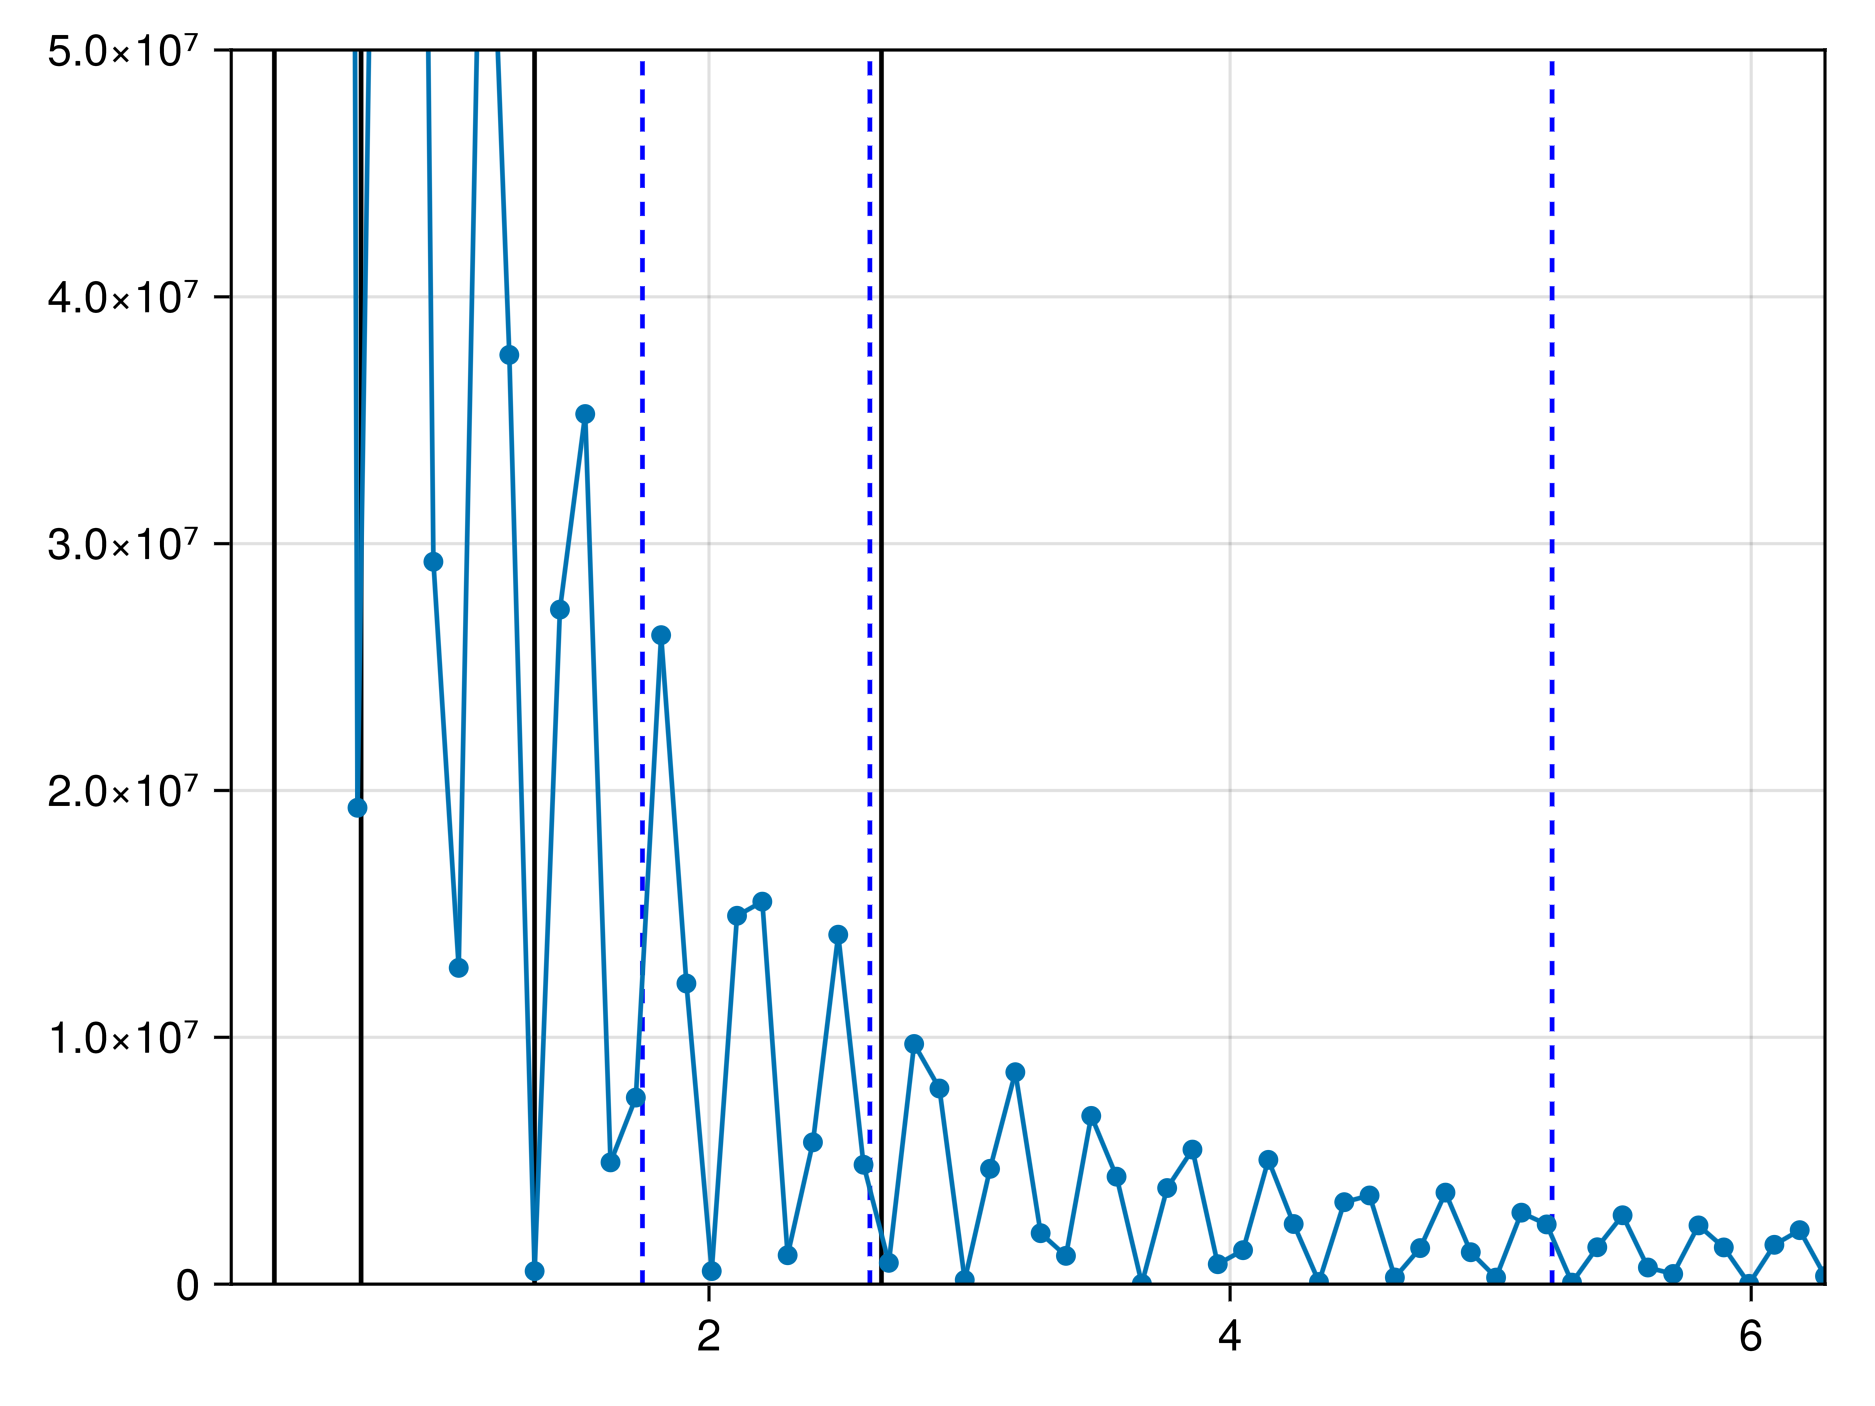
\includegraphics[width=0.9\textwidth]{../Figures/may7/fig_SqCorreccion3_phi5_d_zoom1.png}
    \caption{Factor de estructura con la corrección. \(\phi=5\%\). 
    Las líneas verticales punteadas en azúl están ubicadas en \(|\vec{q}|=2\pi/1.2,~|\vec{q}|=2\pi/(2\cdot1.2),~|\vec{q}|=2\pi/(3\cdot1.2)\).
    Las líneas verticales punteadas en negro están ubicadas en \(|\vec{q}|\in\{2\pi/L,2\pi/L/2,2\pi/L/4,2\pi/L/8,2\pi/L/16\}\).
}
\end{figure}

En este caso creo que está \emph{mejor-ish}.
Estuve analizando el resultado del factor de estructura en desmos y este resultado se parece más al resultado de desmos.
Por otro lado se puede observar que es necesario realizar un sampleo más fino en la magnitud de los vectores de onda.

Por cuestiones de tiempo haré una comparación del resultado con \(2^7\) direcciones y \(2^5\) direcciones para ver si puedo comensar la cantidad de direcciones con la cantidad de experimentos.

Se inició el análisis del factor de estructura para todos los experimentos para el factor de empaquetamiento de 5\% a las 10:10.

\end{document}
